\subsubsection{M\'etodo CFD-DEM}

\noindent
\justify

El acoplamiento entre CFD \textit{(``Computational Fluid Dynamics")} y DEM \textit{(``Discrete Element Method")} busca predecir la interacci\'on fluido-part\'icula. El flujo se resuelve a trav\'es de CFD basado en malla (ver secci\'on \ref{CFD:problema}), mientras que la fase s\'olida es modelada mediante DEM para cada part\'icula sujeta a trav\'es de fuerzas hidrodin\'amicas, fuerzas de cuerpo (como la gravedad) y a trav\'es de fuerzas de contacto; actualizando valores de velocidad y posici\'on conforme a la segunda ley de Newton$^{\cite{Hoomans1996, Xu1997, Tsuji1993}}$. 

\noindent
\justify



\paragraph{Resultados} \label{CFDEM:resultados}

\noindent
\justify

Para la definici\'on de la interacci\'on part\'icula-part\'icula, fluido-part\'icula y part\'icula-muro se emplearon los datos contenidos en el Cuadro \ref{CFDEMdata}.

\begin{table}[h!]
	\centering
	\begin{adjustbox}{max width = 0.45\textwidth}
	\begin{tabular}{|c|c|}
		\hline
		\textbf{Par\'ametro} & \textbf{Valor} \\ \hline
		\multicolumn{2}{|c|}{\textbf{\textit{Generales}}} \\ \hline
		Material & Arena de r\'io \\ \hline
		Tama\~no de part\'icula $[\mu m]$ & 250 \\ \hline
		M\'odulo de Young & $10 ^6$ \\ \hline
		 N\'umero de part\'iculas por segundo & $22300$ \\
		  \hline
		 Velocidad inicial $[m / s]$ & $0.0097$ \\ \hline
		 $\rho [kg/m^3]$ & 1600 \\ \hline
		 $\nu$ & $0.2$ \\ \hline
		 \multicolumn{2}{|c|}{\textbf{\textit{Coeficientes de par de resorte Dashpot}}} \\ \hline
		 $\alpha$ & $0.12$ \\ \hline
		 $\mu$ & $0.52$ \\ \hline
		 Pasos de resoluci\'on de colisi\'on & 12 \\ \hline
	\end{tabular}
	\end{adjustbox}
	\caption{Datos generales para el desarrollo de la simulaci\'on CFD-DEM.}
	\label{CFDEMdata}
\end{table}

\vspace{-0.8cm}

\noindent
\justify

La simulaci\'on num\'erica desarrollada permiti\'o obeservar el comportamiento din\'amico entre las part\'iculas y el solvente; desarroll\'andose el fen\'omeno de sedimentaci\'on desde la entrada de material debido a la baja velocidad de flujo. El diagrama de contorno de velocidades del sistema se puede apreciar en la Figura \ref{CFDEM:vel}.

\begin{figure}[h!]
	\centering
	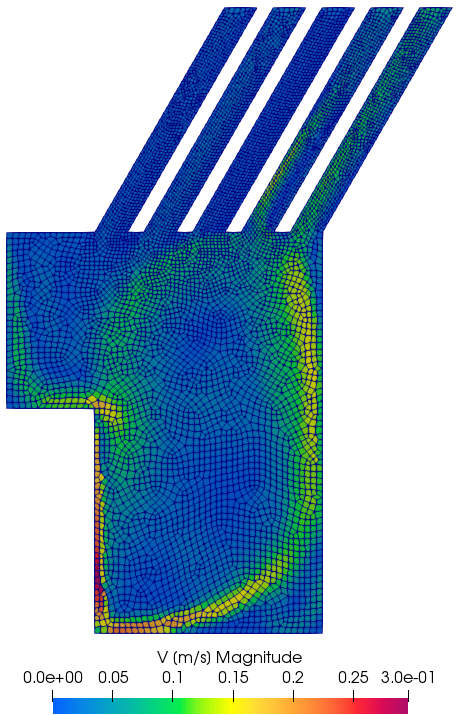
\includegraphics[width=0.31\textwidth]{Images/CFDEM/vel.png}
	\caption{Diagrama de contorno de velocidades del sistema.}
	\label{CFDEM:vel}
\end{figure}

\newpage

\noindent
\justify

El diagrama de contorno de presiones del sistema de sedimentaci\'on se puede apreciar en la Figura \ref{CFDEM:p}.

\begin{figure}[h!]
	\centering
	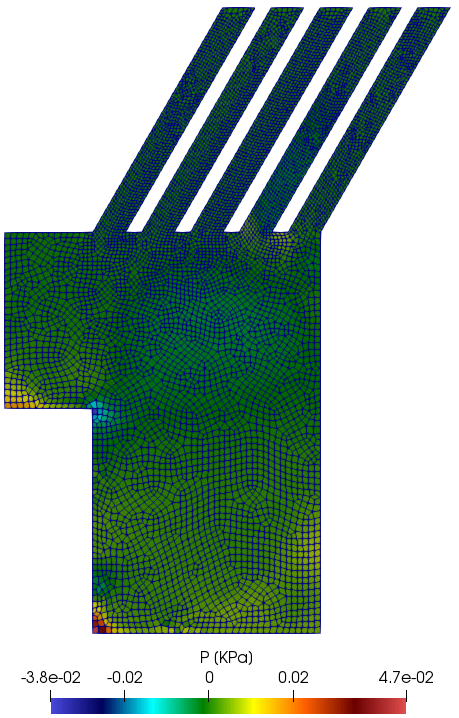
\includegraphics[width=0.31\textwidth]{Images/CFDEM/p.png}
	\caption{Diagrama de contorno de presiones del sistema de separaci\'on de sustancias.}
	\label{CFDEM:p}
\end{figure}

\noindent
\justify

Durante la simulaci\'on, en el que se analizaron $30 [s]$, se apreci\'o el desarrollo de v\'ortices y remolinos debido al reflujo de las part\'iculas, como se aprecia en la Figura \ref{CFDEM:part}.

\begin{figure}[h!]
	\centering
	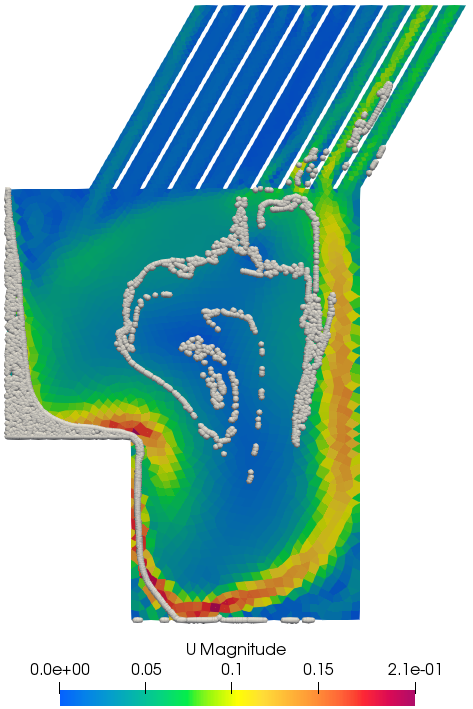
\includegraphics[width=0.355\textwidth]{Images/CFDEM/part.png}
	\caption{Distribuci\'on de part\'iculas de arena sobre el volumen de control durante el segundo $28$ de la simulaci\'on.}
	\label{CFDEM:part}
\end{figure}

\newpage

\paragraph{An\'alisis de resultados} \label{CFDEM:analisis}

\noindent
\justify

Comparando las Figuras \ref{CFD:vel} y \ref{CFDEM:vel}, se puede apreciar c\'omo el solvente cambia la distribuci\'on de velocidades por la sedimentaci\'on sufrida por las part\'iculas de arena, cuya densidad es mayor que la del fluido circundante; raz\'on por la que el solvente tiende a moverse con mayor velocidad en las \'ultimas lamelas en lugar de las primeras, a diferencia de lo observado en la secci\'on \ref{CFD:resultados}. Debido a ello, es posible clasificar a las lamelas por zonas de \textit{``pureza"} durante el proceso de separaci\'on: en donde las primeras seis presentan menor concentrac\'on particular que las \'ultimas cuatro.

\noindent
\justify

La presencia de v\'ortices y remolinos en la simulaci\'on CFD-DEM rectifica la decisi\'on de haber empleado un solucionador basado en \texttt{pimpleFoam}, el cual se adapt\'o para resolver el problema \textit{Euler - Lagrange} (E - L).

\noindent
\justify

Diferente al fen\'omeno apreciado en la Figura \ref{CFD:p}, la distribuci\'on de presiones en la Figura \ref{CFDEM:p} no es sim\'etrica y tiende a presentar sus m\'aximos valores en la zona de congregaci\'on de los sedimentos.

\begin{figure}[h!]
	\centering
	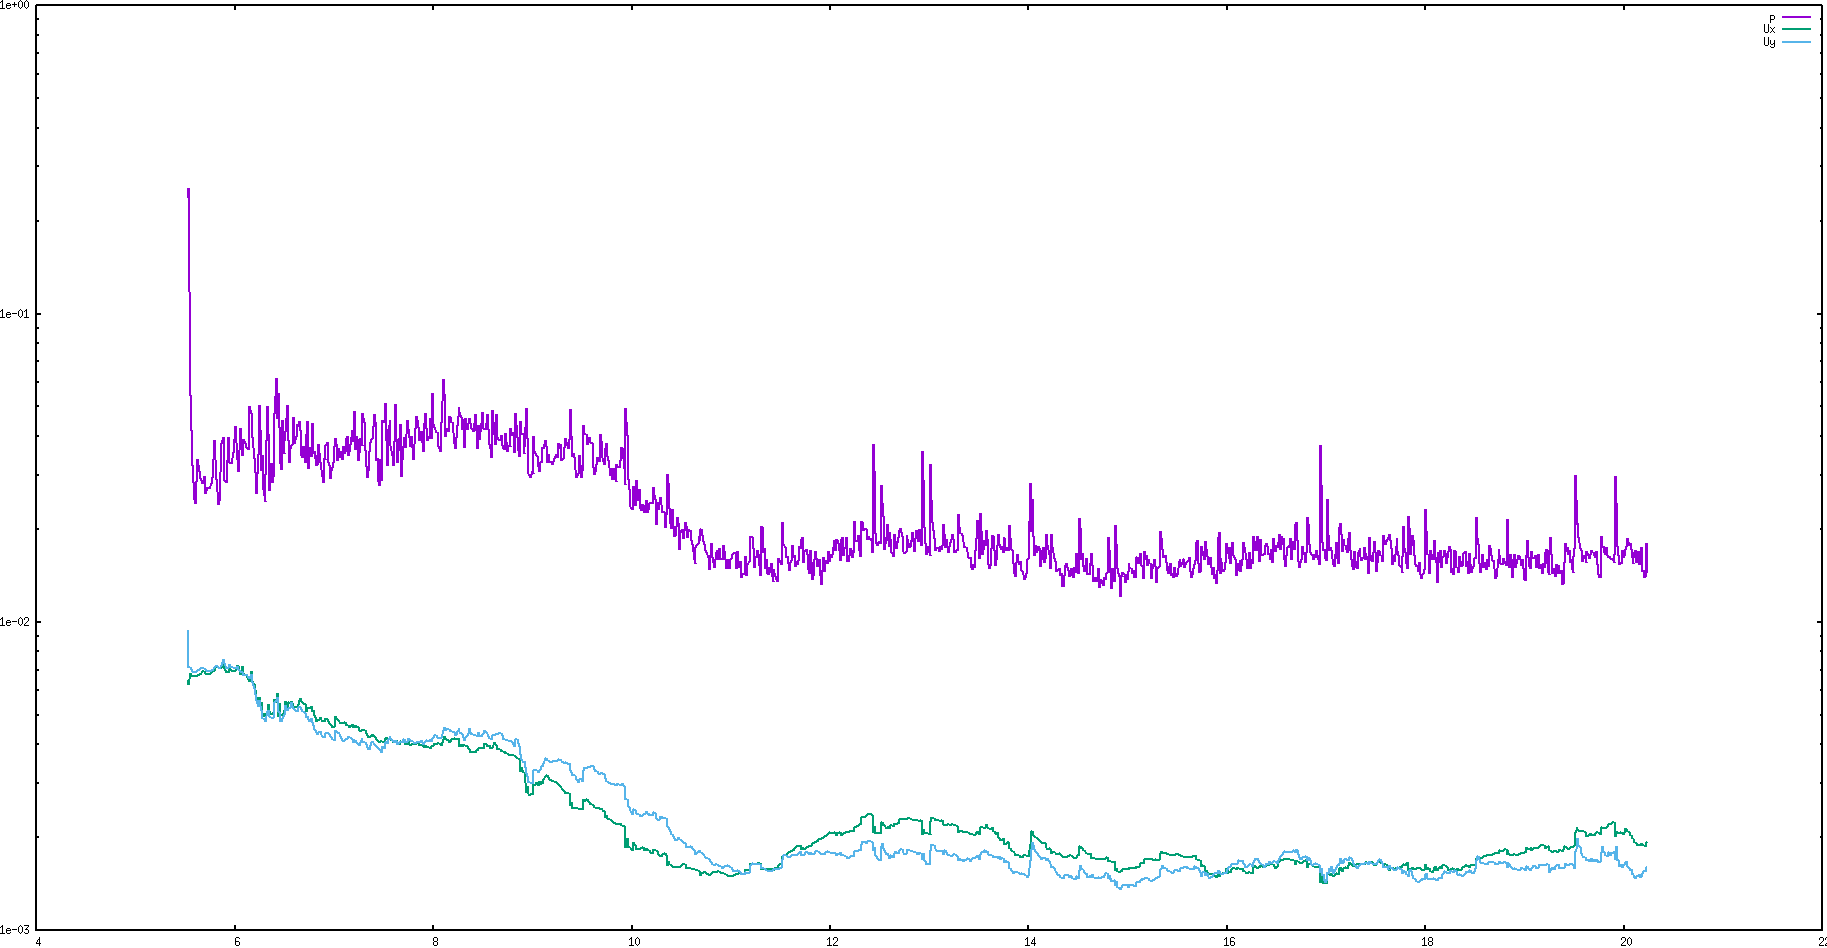
\includegraphics[width=\textwidth]{Images/CFDEM/residuals.png}
	\caption{Monitoreo de residuales en la simulaci\'on CFD-DEM.}
	\label{CFDEM:residuals}
\end{figure}

\noindent
\justify

De la Figura \ref{CFDEM:residuals}, la l\'inea morada corresponde al residual de la presi\'on, la de color cian al residual de la velocidad en $y$ y la de color verde al residual de la velocidad en $x$. El comportamiento de los residuales est\'a directamente relacionado con la magnitud de los errores en la soluci\'on de las ecuaciones gobernantes$^{\cite{Liang2018}}$. Debido al hecho de que tienden a aglomerarse en valores cercanos a cero, son un indicativo de alta precisi\'on del modelo num\'erico implementado. Las variaciones vistas en los residuales de presi\'on se deben a la vorticidad originada por los reflujos consecuentes a la interacci\'on fluido - part\'icula. Durante la simulaci\'on, se observ\'o una estabilizaci\'on en los perfiles de velocidad; raz\'on por la que los residuales $U_x$ y $U_y$ presentan un comportamiento sin fluctuaciones y con peque\~nas variaciones durante el desarrollo del flujo dentro del volumen de control.